\chapter{Prediksi dengan Random Forest}

Untuk pratikum saati ini menggunakan buku \textit{Python Artificial Intelligence Projects for Beginners}\cite{eckroth2018python}. Dengan praktek menggunakan python 3 dan editor anaconda dan library python scikit-learn.
Kode program ada di https://github.com/PacktPublishing/Python-Artificial-Intelligence-Projects-for-Beginners .
Tujuan pembelajaran pada pertemuan pertama antara lain:
\begin{enumerate}
\item
Mengerti implementasi klasifikasi dan teknik evaluasi
\item
Memprediksi spesies burung dengan random forest
\item
Memahami Confusion Matrix.
\end{enumerate}
Tugas dengan cara dikumpulkan dengan pull request ke github dengan menggunakan latex pada repo yang dibuat oleh asisten riset. Kode program menggunakan input listing ditaruh di folder src ekstensi .py dan dipanggil ke latex dengan input listings. Tulisan dan kode tidak boleh plagiat, menggunakan bahasa indonesia yang sesuai dengan gaya bahasa buku teks.

\section{Teori}
Random Forest adalah hasil voting dari beberapa decission tree yang masing-masing memegang atribut yang berbeda. Jadi setiap decission tree spesifik terhadap atribut tersebut yang merupakan bagian kecil dari keseluruhan atribut di data set. Hindari RF jika atribut terlalu sedikit untuk membentuk beberapa tree. Pada praktek kali ini mengggunakan dataset spesies burung yang diambil dari situs 
(http://www.vision.caltech.edu/visipedia/CUB-200-2011.html). Didalamnya terdapat 12.000 foto dari 200 spesies yang berbeda. Yang akan kita pakai untuk RF hanya atribut dari burunynya saja seperti ukuran, bentuk dan warna. Data tersebut diberi label secara manual oleh manusia dengan memanfaatkan jasa dari Amazon's Mechanical Turk.

\subsection{Random Forest}
Pertama dataset kita baca terlebih dahulu.
\begin{lstlisting}[caption=Membaca data file txt,label={lst:fungsisederhana}]
import pandas as pd

# some lines have too many fields (?), so skip bad lines
imgatt = pd.read_csv("data/CUB_200_2011/attributes/image_attribute_labels.txt",
                     sep='\s+', header=None, error_bad_lines=False, warn_bad_lines=False,
                     usecols=[0,1,2], names=['imgid', 'attid', 'present'])

\end{lstlisting}

Melihat sebagian data awal, dengan menggunakan listing \ref{lst:3.1}.

\begin{lstlisting}[caption=Melihat sebagian data awal,label={lst:3.1}]
imgatt.head()
\end{lstlisting}

Melihat jumlah data menggunakan listing \ref{lst:3.2}.
\begin{lstlisting}[caption=Mengetahui jumlah data,label={lst:3.2}]
imgatt.shape
\end{lstlisting}

Merubah atribut menjadi kolom dengan menggunakan pivot layaknya excel. lalu kita cek isinya dengan menggunakan perintah pada listing \ref{lst:3.3}.
\begin{lstlisting}[caption=Pivot dataset,label={lst:3.3}]
imgatt2 = imgatt.pivot(index='imgid', columns='attid', values='present')

imgatt2.head()
imgatt2.shape
\end{lstlisting}


Sekarang kita akan meload jawabannya yang berisi apakah burung itu termasuk dalam spesies yang mana. Dua kolomnya adalah imgid dan label. Dan melakukan pivot yang mana imgid menjadi index yang artinya unik perintahnya ada di listing \ref{lst:3.6}. Lalu kita cek kembali datanya. 
\begin{lstlisting}[caption=membaca dataset label file txt,label={lst:3.6}]
imglabels = pd.read_csv("data/CUB_200_2011/image_class_labels.txt", 
                        sep=' ', header=None, names=['imgid', 'label'])

imglabels = imglabels.set_index('imgid')


imglabels.head()
imglabels.shape
\end{lstlisting}

Karena isinya sama kita bisa melakukan join antara dua data. Sehingga kita akan mendapatkan data ciri dan data jawabannya atau labelnya sehingga bisa dikatekorikan supervised learning. maka perintah untuk menggabungkan kedua data dan kemudian kita melakukan pemisahan antara data set untuk training dan test dengan perintah di listing \ref{lst:3.7}.
\begin{lstlisting}[caption=Menggabungkan field dari dua file terpisah,label={lst:3.7}]
df = imgatt2.join(imglabels)
df = df.sample(frac=1)
\end{lstlisting}

Kemudian drop label yang didepan, dan gunakan label yang paling belakang yang baru di join dengan perintah listing \ref{lst:3.8}.
\begin{lstlisting}[caption=Memisahkan dan memilih label,label={lst:3.8}]
df_att = df.iloc[:, :312]
df_label = df.iloc[:, 312:]
\end{lstlisting}
Kita bisa mengecek isinya dengan perintah listing \ref{lst:3.9}.
\begin{lstlisting}[caption=Melihat isi masing masing data frame,label={lst:3.9}]
df_att.head()
df_label.head()
\end{lstlisting}

Kita bagi menjadi dua bagian, 8000 row pertama sebagai data training sisanya sebagai data testing dengan perintah listing \ref{lst:3.10}.
\begin{lstlisting}[caption=Pembagian data training dan test,label={lst:3.10}]
df_train_att = df_att[:8000]
df_train_label = df_label[:8000]
df_test_att = df_att[8000:]
df_test_label = df_label[8000:]

df_train_label = df_train_label['label']
df_test_label = df_test_label['label']
\end{lstlisting}

Kita panggil kelas RandomForestClassifier. max features diartikan sebagai berapa banyak kolom pada setiap tree dengan perintah listing \ref{lst:3.11}.
\begin{lstlisting}[caption=Instansiasi kelas Random Forest,label={lst:3.11}]
from sklearn.ensemble import RandomForestClassifier
clf = RandomForestClassifier(max_features=50, random_state=0, n_estimators=100)

\end{lstlisting}
Kemudian lakukan fit untuk membangun random forest yang sudah ditentukan dengan maksimum fitur sebanya 50 untuk perpohonnya dengan perintah listing \ref{lst:3.12}.

\begin{lstlisting}[caption=Fitting random forest dengan dataset training,label={lst:3.12}]
clf.fit(df_train_att, df_train_label)
\end{lstlisting}
Hasilnya bisa kita dapatkan dengan perintah predict dengan perintah listing \ref{lst:3.13}.
\begin{lstlisting}[caption=Melihat Hasil prediksi,label={lst:3.13}]
print(clf.predict(df_train_att.head()))
\end{lstlisting}

Untuk besaran akurasinya dengan perintah listing \ref{lst:3.14}
\begin{lstlisting}[caption=Score perolehan dari klasifikasi,label={lst:3.14}]
clf.score(df_test_att, df_test_label)
\end{lstlisting}

\subsection{Confusion Matrix}
Dari RF kita coba petakan ke dalam Confusion Matrix dan lihat hasilnya dengan perintah listing \ref{lst:3.15}.
\begin{lstlisting}[caption=Membuat Confusion Matrix,label={lst:3.15}]
from sklearn.metrics import confusion_matrix
pred_labels = clf.predict(df_test_att)
cm = confusion_matrix(df_test_label, pred_labels)

cm
\end{lstlisting}

Kemudian kita plot dengan perintah
\begin{lstlisting}[caption=Plotting Confusion Matrix,label={lst:3.16}]
import matplotlib.pyplot as plt
import itertools
def plot_confusion_matrix(cm, classes,
                          normalize=False,
                          title='Confusion matrix',
                          cmap=plt.cm.Blues):
    """
    This function prints and plots the confusion matrix.
    Normalization can be applied by setting `normalize=True`.
    """
    if normalize:
        cm = cm.astype('float') / cm.sum(axis=1)[:, np.newaxis]
        print("Normalized confusion matrix")
    else:
        print('Confusion matrix, without normalization')

    print(cm)

    plt.imshow(cm, interpolation='nearest', cmap=cmap)
    plt.title(title)
    #plt.colorbar()
    tick_marks = np.arange(len(classes))
    plt.xticks(tick_marks, classes, rotation=90)
    plt.yticks(tick_marks, classes)

    fmt = '.2f' if normalize else 'd'
    thresh = cm.max() / 2.
    #for i, j in itertools.product(range(cm.shape[0]), range(cm.shape[1])):
    #    plt.text(j, i, format(cm[i, j], fmt),
    #             horizontalalignment="center",
    #             color="white" if cm[i, j] > thresh else "black")

    plt.tight_layout()
    plt.ylabel('True label')
    plt.xlabel('Predicted label')

\end{lstlisting}

 Agar plot sumbunya sesuai dengan nama datanya maka kita set dengan perintah
\begin{lstlisting}[caption=Membaca file classes.txt,label={lst:3.17}]
birds = pd.read_csv("data/CUB_200_2011/classes.txt",
                    sep='\s+', header=None, usecols=[1], names=['birdname'])
birds = birds['birdname']
birds

\end{lstlisting}

Lalu kita plot
\begin{lstlisting}[caption=Plot hasil perubahan label,label={lst:3.18}]
import numpy as np
np.set_printoptions(precision=2)
plt.figure(figsize=(60,60), dpi=300)
plot_confusion_matrix(cm, classes=birds, normalize=True)
plt.show()
\end{lstlisting}



\subsection{Mencoba dengan metode Decission Tree dan SVM}
Kita coba menggunakan Decission tree 
\begin{lstlisting}[caption=Mencoba klasifikasi dengan decission tree dengan dataset yang sama,label={lst:3.19}]
from sklearn import tree
clftree = tree.DecisionTreeClassifier()
clftree.fit(df_train_att, df_train_label)
clftree.score(df_test_att, df_test_label)
\end{lstlisting}
Kita coba menggunakan SVM
\begin{lstlisting}[caption=Mencoba klasifikasi dengan SVM dengan dataset yang sama,label={lst:3.20}]
from sklearn import svm
clfsvm = svm.SVC()
clfsvm.fit(df_train_att, df_train_label)
clfsvm.score(df_test_att, df_test_label)
\end{lstlisting}

\subsection{Pengecekan Cross Validation}
Pengeceken Cross Validation untuk random forest
\begin{lstlisting}[caption=Hasil Cross Validation random forest,label={lst:3.21}]
from sklearn.model_selection import cross_val_score
scores = cross_val_score(clf, df_train_att, df_train_label, cv=5)
# show average score and +/- two standard deviations away (covering 95% of scores)
print("Accuracy: %0.2f (+/- %0.2f)" % (scores.mean(), scores.std() * 2))
\end{lstlisting}
untuk decission tree
\begin{lstlisting}[caption=Hasil Cross Validation Decission Tree,label={lst:3.22}]
scorestree = cross_val_score(clftree, df_train_att, df_train_label, cv=5)
print("Accuracy: %0.2f (+/- %0.2f)" % (scorestree.mean(), scorestree.std() * 2))
\end{lstlisting}
untuk SVM
\begin{lstlisting}[caption=Hasil Cross Validation SVM,label={lst:3.23}]
scoressvm = cross_val_score(clfsvm, df_train_att, df_train_label, cv=5)
print("Accuracy: %0.2f (+/- %0.2f)" % (scoressvm.mean(), scoressvm.std() * 2))
\end{lstlisting}



\subsection{Pengamatan komponen informasi}
Untuk mengetahui berapa banyak tree yang dibuat, berapa banyak atribut yang dipakai dan informasi lainnya menggunakan kode
\begin{lstlisting}[caption=Melakukan Pengamatan komponen informasi,label={lst:3.24}]
max_features_opts = range(5, 50, 5)
n_estimators_opts = range(10, 200, 20)
rf_params = np.empty((len(max_features_opts)*len(n_estimators_opts),4), float)
i = 0
for max_features in max_features_opts:
    for n_estimators in n_estimators_opts:
        clf = RandomForestClassifier(max_features=max_features, n_estimators=n_estimators)
        scores = cross_val_score(clf, df_train_att, df_train_label, cv=5)
        rf_params[i,0] = max_features
        rf_params[i,1] = n_estimators
        rf_params[i,2] = scores.mean()
        rf_params[i,3] = scores.std() * 2
        i += 1
        print("Max features: %d, num estimators: %d, accuracy: %0.2f (+/- %0.2f)" %               (max_features, n_estimators, scores.mean(), scores.std() * 2))

\end{lstlisting}
Dan kita bisa melakukan plot informasi ini dengan kode
\begin{lstlisting}[caption=Plot Komponen informasi agar bisa dibaca,label={lst:3.25}]
import matplotlib.pyplot as plt
from mpl_toolkits.mplot3d import Axes3D
from matplotlib import cm
fig = plt.figure()
fig.clf()
ax = fig.gca(projection='3d')
x = rf_params[:,0]
y = rf_params[:,1]
z = rf_params[:,2]
ax.scatter(x, y, z)
ax.set_zlim(0.2, 0.5)
ax.set_xlabel('Max features')
ax.set_ylabel('Num estimators')
ax.set_zlabel('Avg accuracy')
plt.show()
\end{lstlisting}




\section{Soal Teori}
Praktek teori penunjang yang dikerjakan(nilai 5 per nomor, untuk hari pertama) :
\begin{enumerate}
\item
Jelaskan apa itu random forest, sertakan gambar ilustrasi buatan sendiri.
\item
Jelaskan cara membaca dataset kasus dan artikan makna setiap file dan isi field masing masing file.
\item
Jelaskan apa itu cross validation
\item
Jelaskan apa arti score 44\% pada random forest, 27\% pada decission tree dan 29\%dari SVM.
\item
Jelaskan bagaimana cara membaca confusion matriks dan contohnya memakai gambar atau ilustrasi sendiri.
\item
Jelaskan apa itu voting pada random forest disertai dengan ilustrasi gambar sendiri.
\end{enumerate}

\section{Praktek Program}
Tugas anda adalah,praktekkan dan jelaskan dengan menggunakan bahasa yang mudah dimengerti dan bebas plagiat dan wajib skrinsut dari komputer sendiri masing masing nomor di bawah ini(nilai 5 masing masing pada hari kedua).

\begin{enumerate}
\item buat aplikasi sederhana menggunakan pandas dan jelaskan arti setiap baris kode yang dibuat(harus beda dengan teman sekelas)
\begin{lstlisting}[language=Python]
    #%% 1. Pandas sederhana = 2 dimensional struktur data
    lagu = {'Judul':['Wiped Out', 'Telling Stories', 'Smells Like Teen Spirit', 'Charity'],
            'Band':['Chief State', 'Neck Deep', 'Nirvana', 'Yungblud']} # dictionary yang menampung key dan value nya berupa judul dan band
    
    df = pd.DataFrame(lagu) #kemudian dibuat ke dalam bentuk dataframe yang tampung kedalam sebuah variable dengan nama df
    
    print(df) #untuk menampilkan menggunakan print yang diarahkan ke variable df tadi
\end{lstlisting}
\begin{figure}[!htbp]
    \centering
    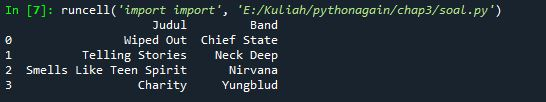
\includegraphics[scale=0.5]{figures/pandasSederhana.JPG}
	\caption{Hasil Pandas Sederhana}
\end{figure}

\item buat aplikasi sederhana menggunakan numpy dan jelaskan arti dari setiap baris kode yang dibuat(harus beda dengan teman sekelas)
\begin{lstlisting}[language=Python]
    #%% 2. Numpy sederhana
    fa = np.array([14,12,20]) # variable fa untuk menampung array 1 dimensi 
    print(fa) #untuk menampilkan hasil variable fa 
\end{lstlisting}
\begin{figure}[!htbp]
    \centering
    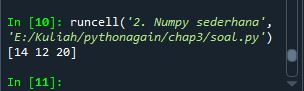
\includegraphics[scale=0.5]{figures/numpySederhana.JPG}
	\caption{Hasil Numpy Sederhana}
\end{figure}

\item buat aplikasi sederhana menggunakan matplotlib dan jelaskan arti dari setiap baris kode(harus beda dengan teman sekelas)
\begin{lstlisting}[language=Python]
    #%% 3. Matplotlib sederhana =  untuk memvisualisasikan data ke dalam bentuk grafik

    x = [1,2,3,5,6,7,3] #variable x untuk menampung semua value dan juga sebagai sumbu x
    y = [1,2,3,3,2,4,5] #variable y untuk menampung semua value dan juga sebagai sumbu y
    
    plt.plot(x, y) #ploting varible x dan y
    
    plt.xlabel('sumbu x') #memberikan label untuk variable x
    plt.ylabel('sumbu y') #memberikan label untuk variabel y
    
    plt.title('Matplotlib sederhana') #memberi title/judul pada plotting yang dibuat
    
    plt.show() #method show digunakan untuk menampilkan plot
\end{lstlisting}
\begin{figure}[!htbp]
    \centering
    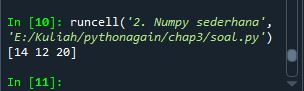
\includegraphics[scale=0.5]{figures/numpySederhana.JPG}
	\caption{Hasil Numpy Sederhana}
\end{figure}

\item jalankan program klasifikasi Random Fores pada bagian teori bab ini. Tunjukkan keluarannya dari komputer sendiri dan artikan maksud setiap luaran yang didapatkan.
\begin{figure}[!htbp]
    \centering
    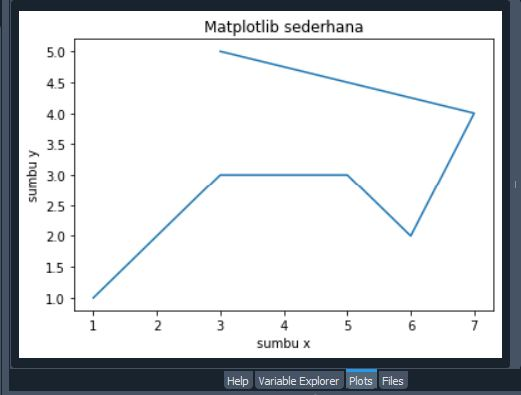
\includegraphics[scale=0.5]{figures/Mtplotlibsederhana.JPG}
	\caption{Hasil Random Forest}
\end{figure}

\newpage
\item jalankan program confusion matrix pada bagian teori bab ini. Tunjukkan keluarannya dari komputer sendiri dan artikan maksud setiap luaran yang didapatkan.
\begin{figure}[!htbp]
    \centering
    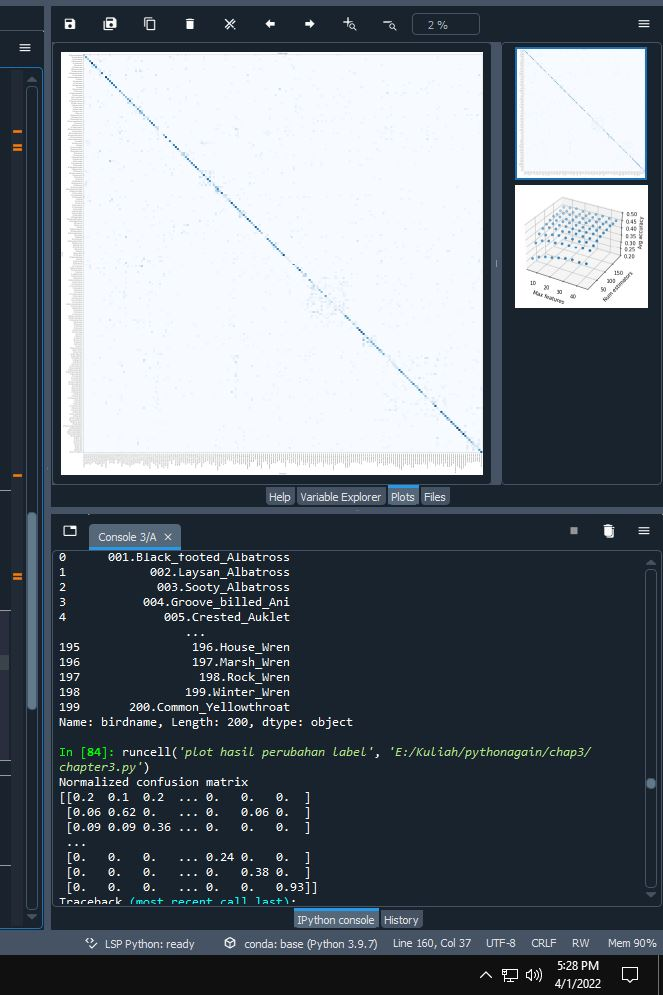
\includegraphics[scale=0.5]{figures/chap3ConfusionMatrix.JPG}
	\caption{Hasil  ConfusionMatrix}
\end{figure}

\newpage
\item jalankan program klasifikasi SVM dan Decission Tree pada bagian teori bab ini. Tunjukkan keluarannya dari komputer sendiri dan artikan maksud setiap luaran yang didapatkan.
\begin{figure}[!htbp]
    \centering
    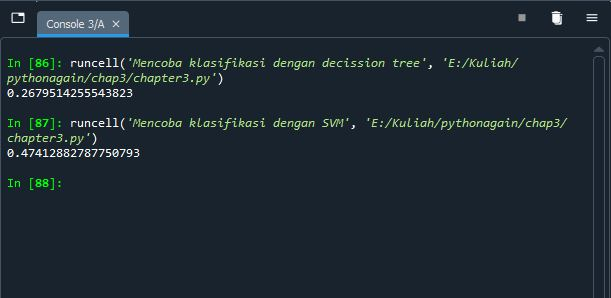
\includegraphics[scale=0.5]{figures/chap3SVMdanDT.JPG}
	\caption{Hasil Klasifikasi DT}
\end{figure}

\item jalankan program cross validaiton pada bagian teori bab ini. Tunjukkan keluarannya dari komputer sendiri dan artikan maksud setiap luaran yang didapatkan.
\newpage
\begin{figure}[!htbp]
    \centering
    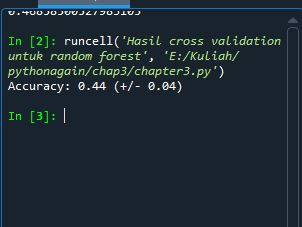
\includegraphics[scale=0.6]{figures/chap3CVjangRF.JPG}
    \caption{Hasil Cross Validation Random Forest}
    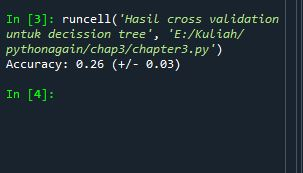
\includegraphics[scale=0.6]{figures/chap3CVjangDT.JPG}
    \caption{Hasil Cross Validation Klasifikasi DT}
    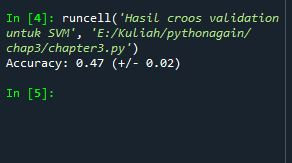
\includegraphics[scale=0.6]{figures/chap3CVjangSVM.JPG}
	\caption{Hasil Cross Validation SVM}
\end{figure}

\item jalankan program pengamatan komponen informasi pada bagian teori bab ini. Tunjukkan keluarannya dari komputer sendiri dan artikan maksud setiap luaran yang didapatkan.
\newpage
\begin{figure}[!htbp]
    \centering
    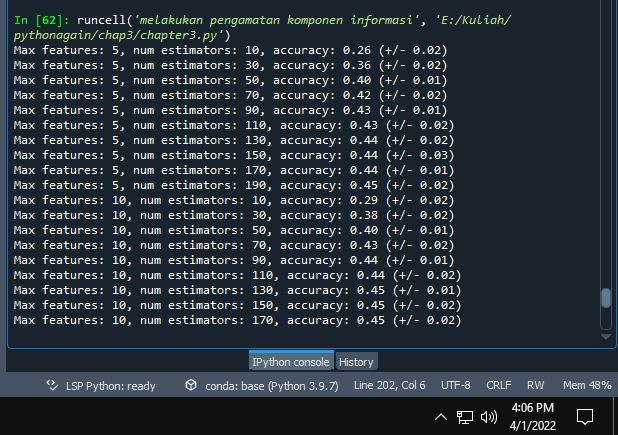
\includegraphics[scale=0.6]{figures/chap3komponeninformasi.JPG}
    \caption{Hasil pengamatan komponen informasi}
    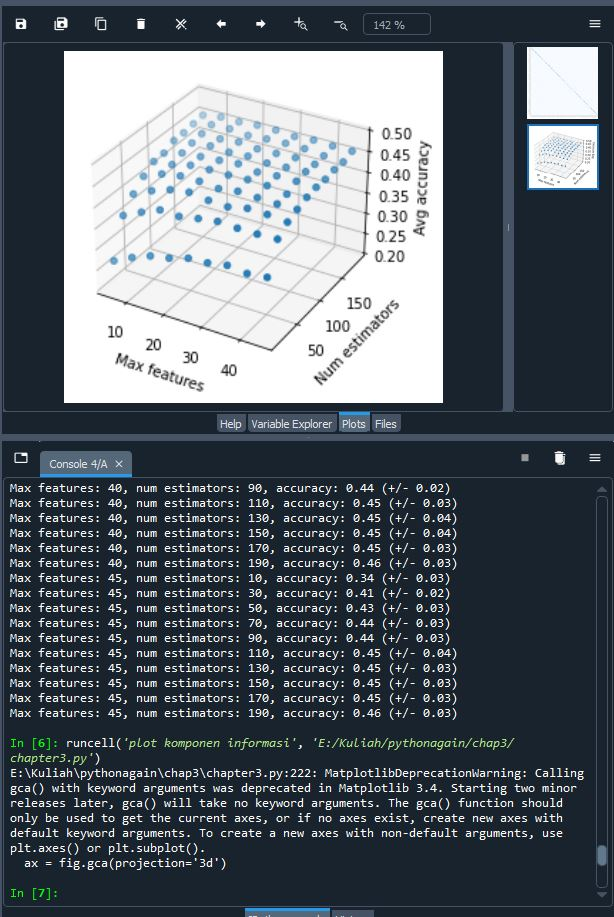
\includegraphics[scale=0.4]{figures/chap3plotkomponen.JPG}
    \caption{Hasil Plot Komponen Informasi}
\end{figure}
\end{enumerate}


\section{Penanganan Error}
Dari percobaan yang dilakukan di atas, error yang kita dapatkan di dokumentasikan dan di selesaikan(nilai 5 per error yang ditangani. Untuk hari kedua):

\begin{enumerate}
	\item skrinsut error
	\item Tuliskan kode eror dan jenis errornya
	\item Solusi pemecahan masalah error tersebut
\end{enumerate}

\section{Presentasi Tugas}
Pada pertemuan ketiga ini, diadakan tiga penilaiain yaitu penilaian untuk tugas mingguan seperti sebelumnya dengan nilai maksimal 100. Kemudian dalam satu minggu kedepan maksimal sebelum waktu mata kuliah kecerdasan buatan. Ada presentasi tugas bab ini dan bab sebelumnya dengan nilai presentasi yang terpisah masing-masing 100. Jadi ada tiga komponen penilaiain pada pertemuan ini yaitu :
\begin{enumerate}
	\item tugas minggu hari ini dan besok (maks 100). pada chapter ini
	\item presentasi decission tree (maks 100). Mempraktekkan kode python dan menjelaskan cara kerjanya.
	\item presentasi Random Forest (maks 100).Mempraktekkan kode python dan menjelaskan cara kerjanya.
\end{enumerate}
Waktu presentasi pada jam kerja di IRC. Kriteria penilaian presentasi sangat sederhana, jika presenter tidak bisa menjawab pertanyaan asisten maka nilai nol. Jika semua pertanyaan bisa dijawab maka nilai 100. Presentasi bisa diulang apabila nilai nol sampai bisa mendapatkan nilai 100 dalam waktu satu minggu kedepan.


